%% This is an example first chapter.  You should put chapter/appendix that you
%% write into a separate file, and add a line \include{yourfilename} to
%% main.tex, where `yourfilename.tex' is the name of the chapter/appendix file.
%% You can process specific files by typing their names in at the 
%% \files=
%% prompt when you run the file main.tex through LaTeX.
\chapter{Fine-tuning BERT for Acceptability Judgements}
\label{chapter:chapter2}
%\chapter{Linguistic analysis of overparametrized models}

Although we have expressed our qualms regarding the probing approach to assessing the KoL of Neural LMs in Section \ref{section:kol}, we believe it important to explore this avenue nonetheless, even if to a limited extent.  Pre-trained Transformer-based models encode a large body of general knowledge, but are poorly optimized for specific natural language tasks out of the box.  Therefore, in order to get optimal downstream task performance, it may be advantageous to fine-tune the pre-trained Transformer model on a downstream task with domain-specific data (\citealp{radford2018improving,devlin2018bert}).

Our task of interest is obtaining acceptability judgements over entire sequences of words from BERT in order to compare them across the LI-Adger minimal pairs under two different criteria.  We do not want to discount the possibility that BERT's performance may improve on either criterion by fine-tuning the model for sequence classification specifically.  We formulate the sequence (acceptability) classification task and training as follows.

When given a sequence of words $s_i$, BERT's final hidden layer will produce an encoded sequence output $h_i$.  Accordingly, we proceed to train a linear output layer that maps via a learned weight matrix $W$ the encoded sequence output $h_i$ to a particular label $c_j$ where $ j \in \{1,0\}$.  The probability of label $c_j$ can then be expressed in terms of the softmax function (Equation \ref{eqn:softmax}), written formally as Equation \ref{eqn:bert_softmax} \citep{sun2019}.
\begin{equation}
    \label{eqn:bert_softmax}
    P(c_j|h) = \mathrm{softmax}(Wh_i)
\end{equation}

We will loosely interpret the output of the softmax in the final layer as the model's \textit{confidence} in a particular label, or how acceptable or unacceptable BERT finds a particular sequence of words to be.  To clarify, although \citet{sun2019} define the output of the softmax in Equation \ref{eqn:softmax} as a true probability, hence why we refer to it as \textit{confidence}, \citet{guo2017calibration} among others have found that in order for the softmax output of a neural network to be considered a true probability or confidence, it must be calibrated to the true correctness likelihood via other post-processing methods currently unavailable to us.  For example, there is currently no complete theory of the gradient nature of acceptability that can produce the gradient acceptability score for a given sentence on demand \citep{sprouse2012assessing}.  However, without confidence calibration, \citet{guo2017calibration} find the softmax output of modern neural networks often overestimates the true underlying probabilities.  Conversely, when BERT is used to predict the probability of a token (Masked Language Modeling - MLM), a similar softmax operation is performed to yield what is considered the true probability of the target token.  We do not adopt a particular stance on the matter and will simply use the italicized term \textit{confidence} to refer to the softmax output as formulated in Equation \ref{eqn:bert_softmax} by \citet{sun2019}.

\section{BERT pilots the BLiMP}
\label{section:2.1}
Over the course of this chapter and the remainder of this thesis, we will be working with Bidirectional Encoder Representations from Transformers (BERT; \citet{devlin2018bert}).  We determined BERT to be the ideal model to test due to the growing body of research attributing ever greater KoL to BERT. \citet{warstadt2019linguistic} have already shown high Matthews Correlation Coefficient (MCC; \citealp{matthews1975comparison}) scores between the expert acceptability labels for the sentences in the Corpus of Linguistic Acceptability (CoLA; \citealp{warstadt2019neural}) and BERT$_\mathrm{CoLA}$ models' predictions.  These researchers have gone on to show with a grammatically annotated CoLA analysis set that BERT$_\mathrm{CoLA}$ models exhibit very strong positive MCC scores on multiple syntactic features.  For example, they claim BERT exhibits strong knowledge of complex or noncanonical argument structures such as ditransitives and passives, and has a distinct advantage over baseline performance on sentences with long-distance dependencies such as questions.  %Indeed \citet{warstadt2020can} have even suggested that BERT is able to acquire a structural bias from raw linguistic data, putting into question the argument of the Poverty of the Stimulus.  
Additionally, \citet{Manning2020} have approximated sentence tree structures by linearly transforming BERT's learned representations into a metric that captures parse tree distances.  Finally, \citet{salazar2020} used the raw psuedo-log-likelihood (PLL; \citealp{wang2019bert,shin2019effective,salazar2020}) from the out-of-the-box BERT$_\mathrm{MLM_{large-cased}}$ to evaluate its KoL using the BLiMP benchmark and found it to correctly predict 84.8\% of the minimal pairs in BLiMP, thereby beating GPT-2 by 4.2\% and almost reaching the human baseline at 88.6\%.  As we will demonstrate below, we do not align ourselves with many of the claims we have reviewed here regarding the KoL encoded in BERT. Nonetheless, we believe it important to provide background for the \textit{claims} that have recently been made in the field.\footnote{For a recent review of the knowledge of language that has been attributed to BERT, see \textit{A Primer in BERTology: What We Know About How BERT Works}, \citep{rogers2021primer}} %While we do not align ourselves with many of the claims we have reviewed here regarding the KoL encoded in BERT, as we will soon demonstrate, we believe it important nonetheless to provide background for the \textit{findings} that have recently been made in the field.\footnote{For a recent review of the knowledge of language that has been attributed to BERT, see \textit{A Primer in BERTology: What We Know About How BERT Works}, \citep{rogers2021primer}}  
We will take the information provided here as the baseline level of performance we will expect from BERT moving forward: in other words, we do not believe it unfair given these results to \textit{a priori} expect BERT to exhibit the same or a similar level of gradience in acceptability judgements across minimal pairs to that of humans.



\section{BERT drinks the CoLA}
\label{section:2.2}
In order to provide BERT with the best possible chance of achieving maximum performance in our proposed test of KoL using the LI-Adger dataset and the ADC, we begin our analyses of BERT by first replicating the results observed by \citet{warstadt2019linguistic}(henceforth W\&B 2019).  This replication serves two purposes: to ensure that our training regime did not inadvertently cripple BERT in any meaningful way, and to have an objective data point of how performance on phenomena attributed to BERT such as noncanonical argument structures, as W\&B argued, translates to performance on the ADC.

We use the Huggingface Transformers library \citep{wolf-etal-2020-transformers} to fine-tune three pre-trained versions of BERT in order to be comprehensive in our coverage: 10 random seeds of BERT$_\mathrm{CoLA_{base-uncased}}$, 20 random seeds of BERT$_\mathrm{CoLA_{large-uncased}}$, and 20 random seeds of BERT$_\mathrm{CoLA_{large-cased}}$.  Here we note a slight divergence from the authors in methodology.  W\&B 2019 noted they trained 20 random restarts of BERT$_\mathrm{CoLA_{large}}$ (we suspect the cased version) and discarded 5 out of the 20 restarts because they were degenerate, i.e. those restarts yielded an MCC of zero on the CoLA test set.  Instead of training a fixed number of seeds and then discarding the degenerate ones, we continued training seeds until we reached 20 nondegenerate random restarts of BERT$_\mathrm{CoLA_{large-uncased}}$ and BERT$_\mathrm{CoLA_{large-cased}}$.  

We recreate in Table \ref{tab:table_6} below an updated version of the table of MCC scores on the CoLA test set presented by W\&B both in 2018 and 2019.  We add a column to indicate the authors responsible for training the model and include our three trained models in the comparison.  Additionally, we include two models submitted by Jacob Devlin to the \hyperref[https://gluebenchmark.com/leaderboard]{GLUE Leaderboard} for additional points of comparison, although we assume the scores presented in the leaderboard are the maximum MCC scores achieved by the models on the CoLA out-of-domain test set.

\begin{table}[h]
    \centering
    \ra{1.3}
    \begin{tabular}{@{}lcccl@{}}
    \toprule
    \textbf{Model${_\mathrm{CoLA}}$} & \textbf{Mean (STD)} & \textbf{maximum} & \textbf{Ensemble} & \textbf{Authors} \\
    \midrule
    CoLA baseline & 0.320 (0.007) & 0.330 & 0.320 & W\&B 2019\\
    GPT & 0.528 (0.023) & 0.575 & 0.567 & W\&B 2019 \\
    \textbf{BERT$_{\mathrm{large}}$} & \textbf{0.582 (0.032)} & \textbf{0.622} & \textbf{0.601} & \textbf{W\&B 2019}\\
    Human & 0.697 (0.042) & 0.726 & 0.761 & Warstadt et al. 2018\\
    \midrule
    BERT$_{\mathrm{base-uncased}}$ & 0.478 (0.018) & 0.514 & 0.522 & H\'ector \& friends \\
    BERT$_{\mathrm{large-uncased}}$ & 0.542 (0.019) & 0.583 & 0.578 & H\'ector \& friends \\
    \textbf{BERT$_{\mathrm{large-cased}}$} & \textbf{0.574 (0.026)} & \textbf{0.613} & \textbf{0.588} & \textbf{H\'ector \& friends} \\
    \midrule
    BERT$_{\mathrm{base}}$ & 0.521* (N/A) & 0.521* & 0.521* & Jacob Devlin \\
    \textbf{BERT$_{\mathrm{large}}$} & \textbf{0.605* (N/A)} & \textbf{0.605*} & \textbf{0.605*} & \textbf{Jacob Devlin} \\
    \bottomrule
    \end{tabular}
    \caption[MCC scores on the CoLA out-of-domain test set]{Replication of \citet{warstadt2019linguistic} with our trained BERT$_\mathrm{CoLA}$ models for comparison.  Performance (MCC) on the CoLA test set, including mean over restarts of a given model with standard deviation, maximum over restarts, and majority prediction over restarts.  We include the BERT$_\mathrm{CoLA}$ scores on the GLUE leaderboard for the CoLA task submitted by Jacob Devlin for further points of reference.}
    \label{tab:table_6}
\end{table}

Our mean MCC scores for BERT$_\mathrm{CoLA_{large-cased}}$ were within error margins of the BERT$_\mathrm{CoLA_{large}}$ model reported by W\&B 2019.  Additionally, the maximum MCC score achieved here by BERT$_\mathrm{CoLA_{large-cased}}$ beat the score posted by Jacob Devlin on the GLUE Leaderboard, and was less than 0.01 away from the maximum MCC score posted by W\&B's  BERT$_\mathrm{CoLA_{large}}$.  We consider these results to be strongly indicative of successful replication, given the known stochastic variation in such models, and proceed to conduct the remainder of the linguistic analyses presented by W\&B 2019 using the CoLA analysis set.  However, we focus our analyses exclusively on the three  BERT$_\mathrm{CoLA}$ models we trained, and do not replicate the results of the other models, as they are not the focus of this thesis.

When we consider only the major features in the CoLA analysis set, the replication trial seems even more promising.  In Figure \ref{fig:bert_mcc_scores_cola_major_features} below we replicate the first figure in W\&B 2019, which shows model performance by major syntactic feature in the CoLA analysis set.  We deviate slightly from the authors when plotting mean MCC performance.  While they use dashed lines to show MCC performance on the entire CoLA development set, we use them to show MCC performance on the CoLA out-of-domain test set as a follow up to the MCC scores presented in Table \ref{tab:table_6}.

\begin{figure}[h]
    %\centering
    \makebox[\textwidth][c]{
        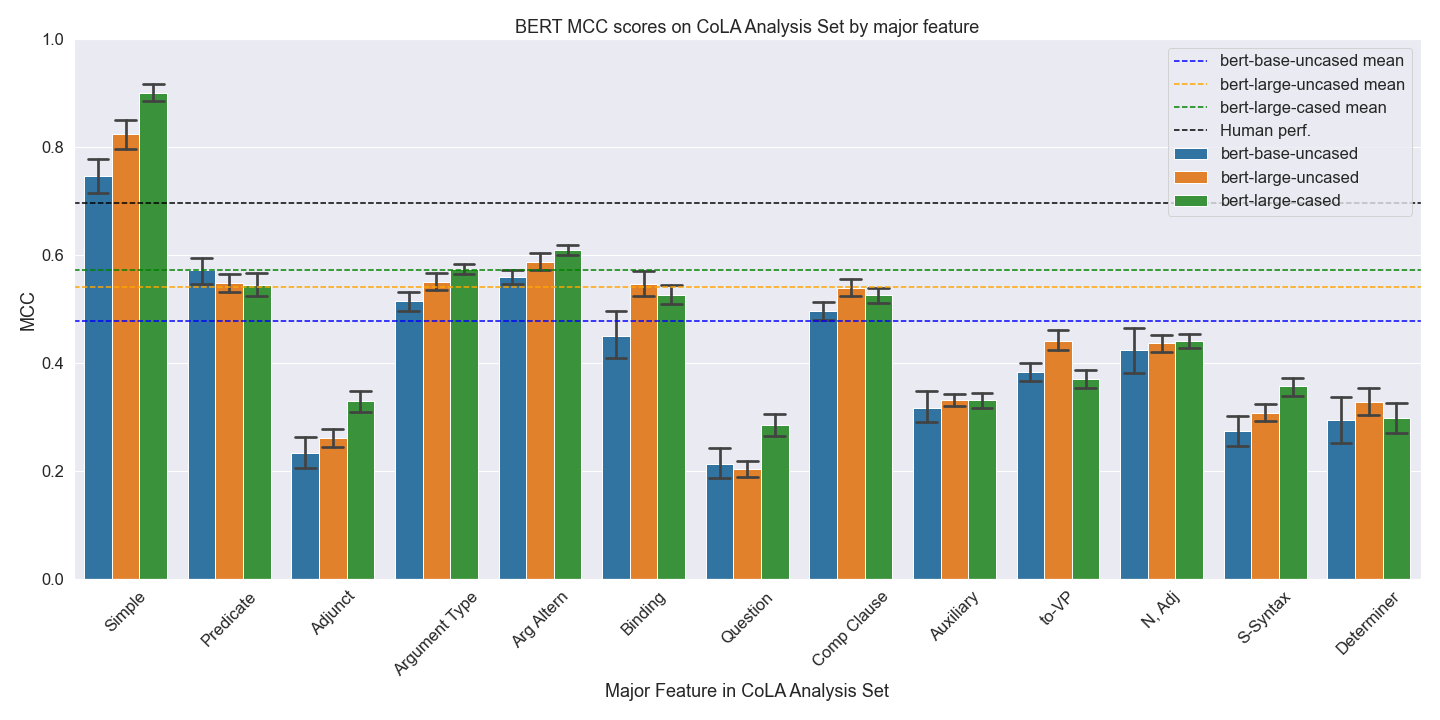
\includegraphics[scale=0.3]{templates/figures/bert_mcc_scores_cola_major_features.png}
    }
    \caption[BERT$_\mathrm{CoLA}$ MCC scores on CoLA Analysis Set by major feature]{Replication of \citet{warstadt2019linguistic} with our BERT$_\mathrm{CoLA}$ models for comparison.  Performance (MCC) on CoLA analysis set by major feature.  Dashed lines show mean performance on the CoLA out-of-domain test set.  From left to right, performance for each feature is given for base-uncased, large-uncased, and large-cased.}
    \label{fig:bert_mcc_scores_cola_major_features}
\end{figure}

Unfortunately, the major features in the CoLA analysis set are where our successful replication ends.  By that we mean that studying the finer-grained minor features in the analysis set reveals what the MCC scores on the test set and major features have obscured.  Much like Figure \ref{fig:bert_mcc_scores_cola_major_features}, we replicate the second figure in W\&B 2019 in Figure \ref{fig:bert_mcc_scores_cola_minor_features}, but again using the average CoLA out-of-domain test set MCC scores presented in Table \ref{tab:table_6} as the horizontal dashed lines.

\begin{figure}[h!]
    %\centering
    \makebox[\textwidth][c]{
        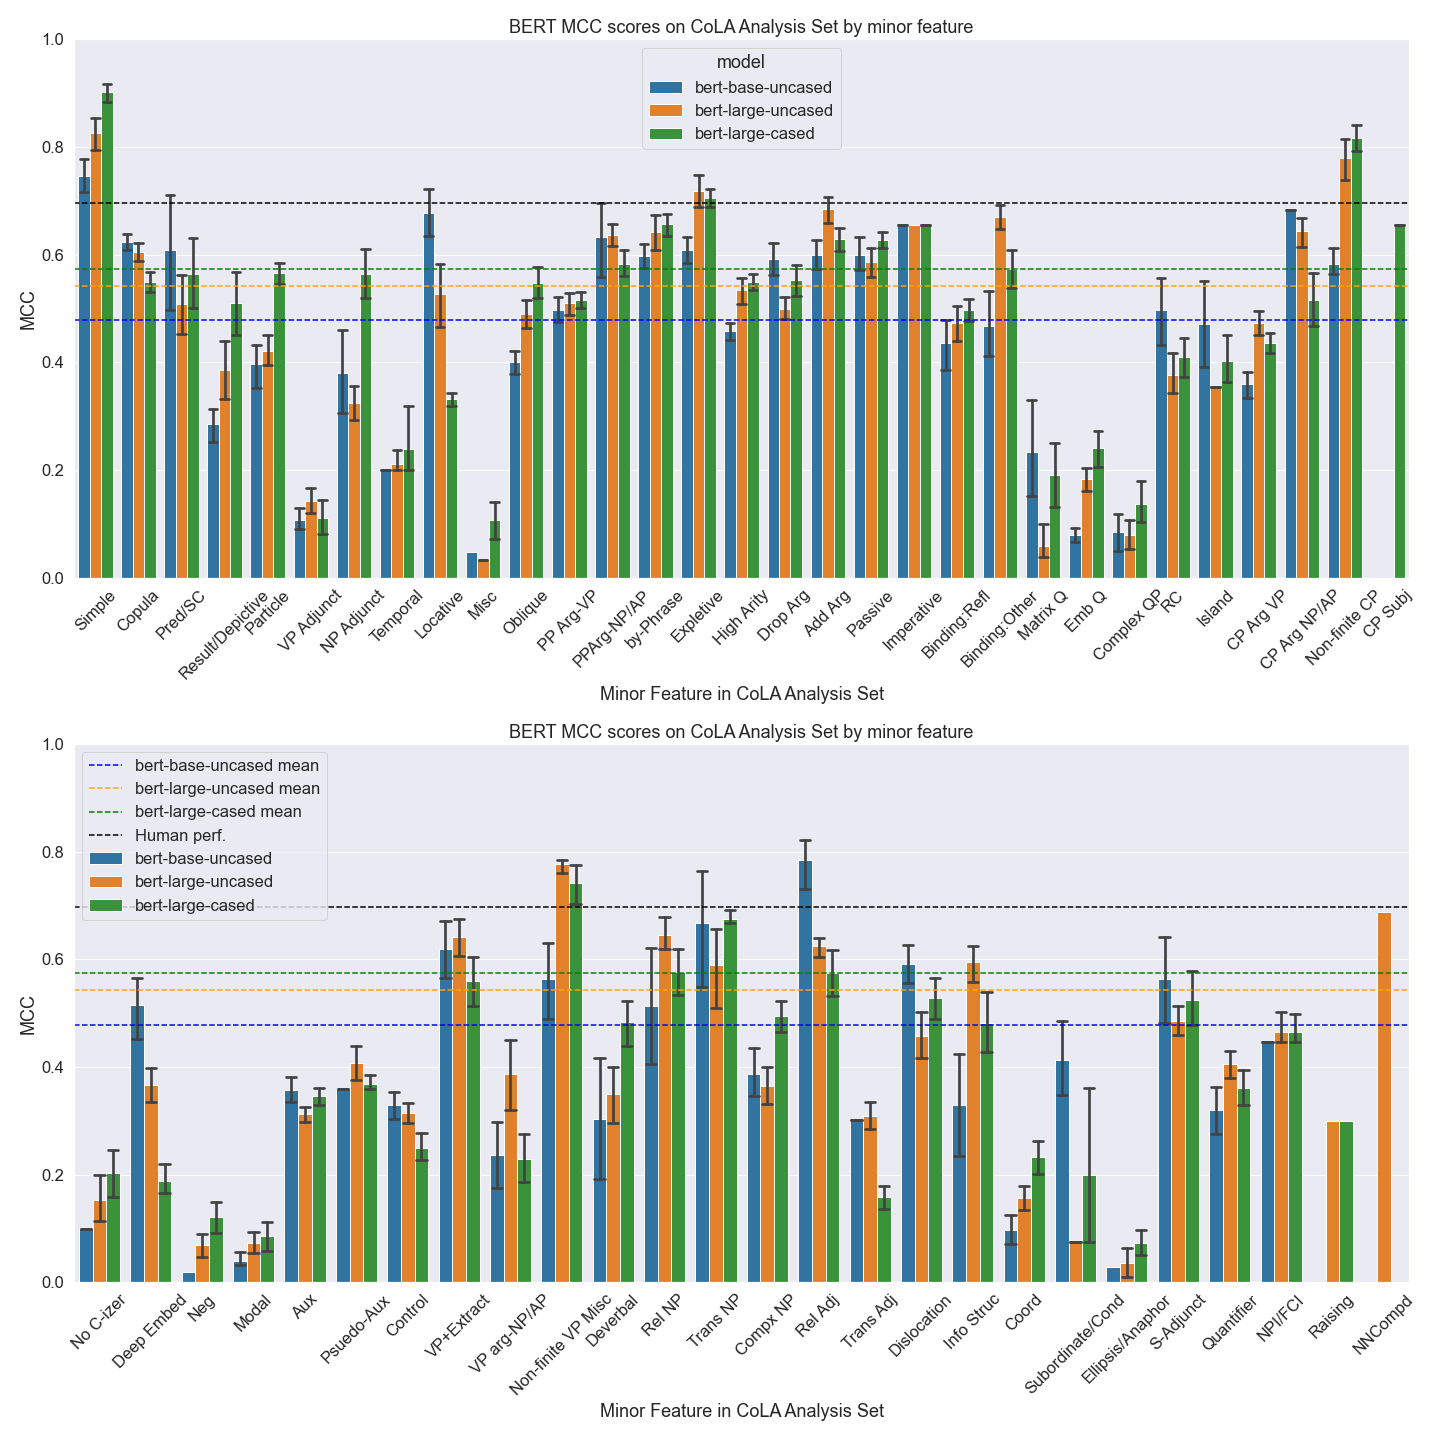
\includegraphics[scale=0.3]{templates/figures/bert_mcc_scores_cola_minor_features.png}
    }
    \caption[BERT$_\mathrm{CoLA}$ MCC scores on CoLA Analysis Set by minor feature]{Replication of \citet{warstadt2019linguistic} with our trained BERT$_\mathrm{CoLA}$ models for comparison.  Performance (MCC) on CoLA analysis set by minor feature.  Dashed lines show mean performance on the CoLA out-of-domain test set.  From left to right, performance for each feature is given for base-uncased, large-uncased, and large-cased.}
    \label{fig:bert_mcc_scores_cola_minor_features}
\end{figure}

The added resolution of the minor features reveals somewhat erratic behavior from the three different BERT models.  For one, we observe degenerate performance (MCC = 0) on a number of features, but most notably sentences that contain Complement Clause Subjects (CP Subj), Raising, or Noun-Noun Compounds (NNCompd) toward the right-hand side of Figure \ref{fig:bert_mcc_scores_cola_minor_features}.  Thankfully, we only see this degenerate behavior from BERT$_{\mathrm{CoLA_{large-cased}}}$ in NNCompd, but also observe very low MCC scores for a handful of other features.  Most notably, the BERT$_{\mathrm{CoLA}}$ models perform the worst on the Question major feature in Figure \ref{fig:bert_mcc_scores_cola_major_features}, which also translates to poor performance on Matrix Questions (Matrix Q) and Embedded Questions (Emb Q).  Other underperforming minor features of note are the  Miscellaneous Adjuncts (Misc), Modal Verbs (Modal) and Negation (Neg).  We believe this to be a manifestation of the underspecification phenomenon identified by \citet{d2020underspecification}, where near identical performance on I.I.D. test sets is nonetheless met with different combinations of spurious and meaningful correlations acquired during training.  Although we do not proceed to investigate the extent of this underspecification behavior as it pertains to W\&B 2019, we do investigate to what extent this may be reflected when testing performance on the LI-Adger dataset.

Given the positive MCC results by BERT$_\mathrm{CoLA_{large-cased}}$ on the CoLA out-of-domain test set, CoLA analysis set major features, and even many of the minor features in the analysis set, we are satisfied with the performance of our BERT$_\mathrm{CoLA_{large-cased}}$ model's performance.  Accordingly, we select the random restart that yielded the maximum MCC score reported in Table \ref{tab:table_6} as the model to be studied in our later analyses.  Lastly, we have grounds to believe our failure to replicate exact results on the CoLA analysis set's minor features is not the fault of our training regime or choice of hyperparameters, but rather a consequence of the overparametrization that is characteristic of the BERT models, and almost certainly all neural LMs \citep{d2020underspecification}.

\section{BERT has too much to drink}
\label{section:bert_instability}

The volatility in the three BERT$_\mathrm{CoLA}$ models' predictions revealed by our attempts to replicate the results of \citet{warstadt2019linguistic} warrants further investigation.  As we briefly alluded to in Section \ref{section:2.2}, we do not intend to assess the degree of instability in the CoLA analysis set, nor do we wish to make claims regarding the validity of the KoL attributed to BERT as a result of \citeauthor{warstadt2019linguistic}'s findings.  Our interest here is simple: we want to know how and to what degree the overparametrization of the BERT$_\mathrm{CoLA}$ models may affect the results we observe when obtaining acceptability judgements from BERT$_\mathrm{CoLA}$ on the LI-Adger sentences before applying the Acceptability Delta Criterion.

Due to limited computational resources, we conduct the following experiment.  We initialize a single instance of pre-trained BERT$_{\mathrm{base-uncased}}$ with a linear classification head as expressed in Equation \ref{eqn:bert_softmax} at the beginning of the chapter.  This is the only point in the experiment where a model is initialized, so the weight matrix $W$ in the linear output layer will always have the exact same starting weights.  Next, we make a full copy of the model in order to keep the base initialization without any fine-tuning, and perform fine-tuning on the second copy using the CoLA.  However, before performing the fine-tuning, we shuffle the order of the training data according to one random seed.  After the fine-tuning process, we gather a categorical acceptability prediction from BERT$_\mathrm{CoLA_{base-uncased}}$ for each sentence in the LI-Adger sentence by selecting the label with the highest softmax output.  I.e. for the sentence \textit{Colorless green ideas sleep furiously} ($s_i$), one random seed of BERT$_\mathrm{CoLA_{base-uncased}}$ outputs a softmax value of 0.168 for the the unacceptable label ($P(c_j=0|h_i) = 0.168$), and a softmax value of 0.832 for the acceptable label ($P(c_j=1|h_i) = 0.832$). Therefore, we determine the model's prediction for that sentence to be 1.0 (acceptable).  We express the model's output $out_i$ more succinctly as follows:
\begin{equation}
    out_i = \argmax_{c_j \in \{0, 1\}}\bigg[P(c_j|h_i)\bigg]
\end{equation}
Although we change this paradigm for later analyses, we continue to use the categorical output for this particular experiment because it allows us to calculate performance using MCC as in the CoLA out-of-domain test set, which is where we first identified this particular instability.

We repeat the process of cloning BERT$_{\mathrm{base-uncased}}$ and fine-tuning the copy with the reshuffled CoLA training set 200 times.  That is, the exact same BERT model is trained on the same data, but shuffled into 200 different orders.  Each time we collect the fine-tuned model's categorical predictions for the sentences in the LI-Adger dataset, we compare them to the previous seed's predictions.  Every sentence whose predicted label changes between the previous and current random seed is considered an ``Acrobatic Sentence" due to its exhibited \textit{fipping} behavior in response to a reordering of the training data.  For the sake of consistency, we name the sentences whose predictions remain constant the ``Unathletic Sentences," because they do not \textit{flip} back and forth.  We plot the percentage of the LI-Adger sentences that fall into the set of Acrobatic Sentences as a function of the number of different training orders used to fine-tune BERT$_\mathrm{CoLA_{base-uncased}}$ in Figure \ref{fig:bert_stability_testing}.  We additionally plot the baseline accuracy of a majority-class predictor.

\begin{figure}[h]
    %\centering
    \makebox[\textwidth][c]{
        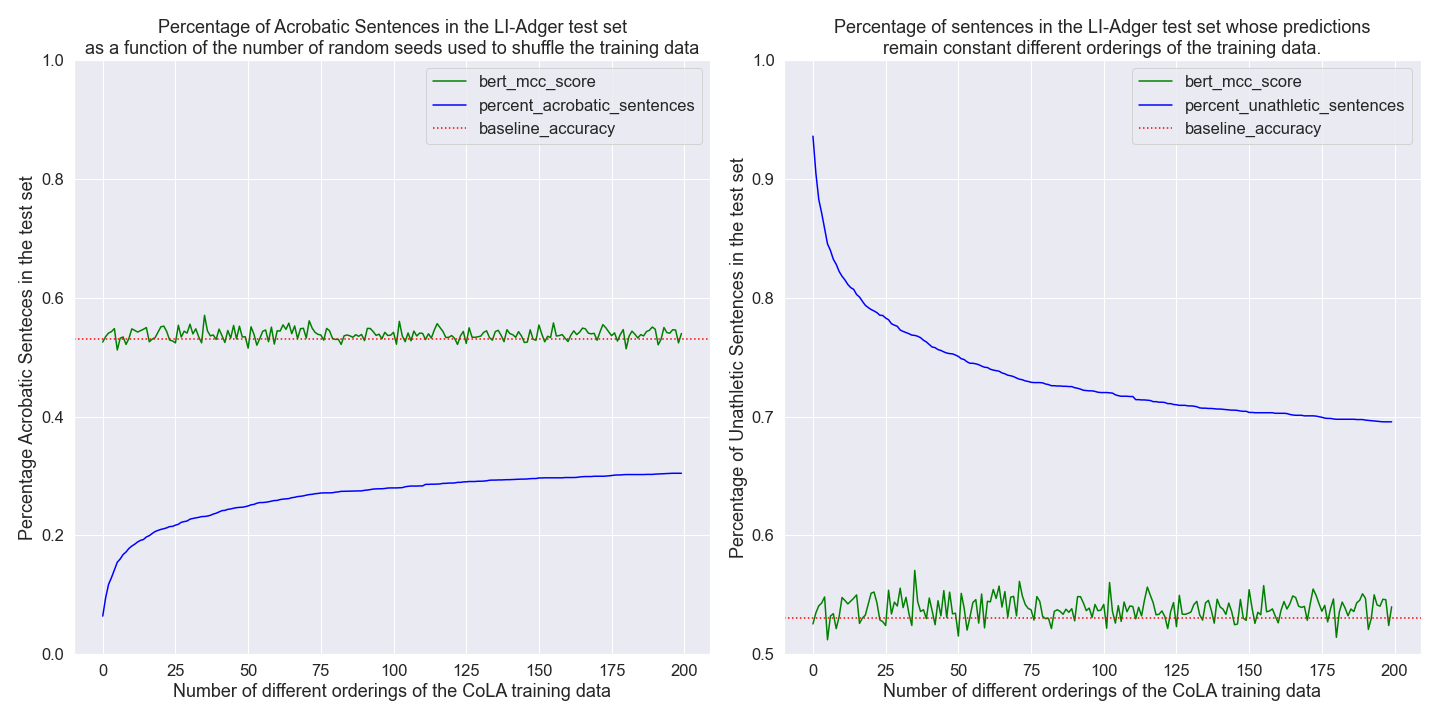
\includegraphics[scale=0.3]{templates/figures/bert_stability_testing.png}
    }
    \caption[Percentage of Acrobatic Sentences in the LI-Adger test set]{As the same initialization of BERT$_\mathrm{CoLA_{base-uncased}}$ is fine-tuned in different random orders, the percentage of sentences in the test set that become Acrobatic Sentences (left) and the percentage of sentences whose predicted labels remain constant (Unathletic Sentences--right). The MCC score achieved by BERT on the LI-Adger dataset at each random seed is plotted in green.  The baseline accuracy of a majority-class predictor is plotted in orange.}
    \label{fig:bert_stability_testing}
\end{figure}

The pattern of instability in Figure \ref{fig:bert_stability_testing} has important negative implications for the strength of any conclusions that can be drawn regarding BERT if it needs to be fine-tuned as part of the experiment.  Recall this instability arises from the fundamentally underdetermined system of equations the model is trying to solve, which by nature either have no solutions or infinitely many solutions.  By having more parameters than data points, BERT, as well as any other such overparametrized model, is able to settle on an unknown number of spurious correlations that may yield good performance on I.I.D. test sets \citep{d2020underspecification}.  Figure \ref{fig:bert_stability_testing} shows that while BERT$_\mathrm{CoLA_{base-uncased}}$ has a relatively constant MCC score on the LI-Adger dataset, it changed its predictions for 1272 out of the 4178 total sentences in the LI-Adger dataset.  What is more sobering is the fact that we performed this test with the BERT$_{\mathrm{base-uncased}}$ model, the version of BERT with the fewest parameters.  Although we do not conduct the same test with BERT$_{\mathrm{large-cased}}$ out of a lack of computational resources, we have no reason to believe this instability will be any less pronounced.  On the contrary, because we are effectively tripling the number of free parameters (from 110M in BERT$_{\mathrm{base}}$ to 340M in BERT$_{\mathrm{large}}$) in an already underdetermined system of equations, we expect nothing other than an even more severe instability.

At this point we can summarize what this implies for our Acceptability Delta Criterion test using the LI-Adger dataset.  We briefly discussed in Section \ref{section:kol} why we do not believe probing to be the best approach to assessing the KoL of neural LMs.  The results observed in Figure \ref{fig:bert_stability_testing} are strong evidence for the lack of reliability of such experiments.  However, we will proceed to study the performance of BERT$_\mathrm{CoLA}$ models on the LI-Adger dataset under the Acceptability Delta Criterion nonetheless.  We will not yet dismiss the argument that BERT must be fine-tuned for sequence classification in order to perform its best \citep{sun2019}.  However, we will evaluate BERT by adopting some of the recommendations of D'Amour et al. 2020.

Let us momentarily set aside the scientific question and consider BERT for what it is: an engineering achievement capable of state-of-the-art performance in deployment of multiple different NLP services and tasks such as Google Search.  If we take the LI-Adger dataset as an example of data that will be observed in deployment, then we cannot select a BERT model to evaluate according to MCC performance on the LI-Adger dataset.  After all, if one had access to the data that that will be seen in deployment... what would be the point of all the research that has been conducted for Machine Learning models to generalize beyond the training data?  Consequently, we select the BERT$_\mathrm{CoLA}$ model to evaluate according to MCC performance on the CoLA out-of-domain test set, and then evaluate its performance on an entirely unseen LI-Adger dataset.

The last point we wish to make is that we select a \textbf{single} model out of the multiple random restarts of each of the BERT$_\mathrm{CoLA}$ models instead of averaging predictions across them.  This is in part because the ML pipeline typically selects the model that best performs on the held-out test set and uses it in deployment.  The principal reason for this approach, however, is that we wish to evaluate the KoL contained in the model.  By averaging the predictions of multiple different random restarts of the same model, especially with the degree of instability observed in Figure \ref{fig:bert_stability_testing}, we might mask anything meaningful that we could learn about the models, because the test would amount to evaluating the average of many different spurious correlations, even if it results in better performance overall.


\section{Benchmarking with the LI-Adger Dataset}
\label{section:2.4}

Having evaluated all the models on the CoLA out-of-domain test set, we select the best performing random restart of each model to evaluate under the Acceptability Delta Criterion using the LI-Adger dataset.  However, before applying the Acceptability Delta Criterion, we treat the LI-Adger dataset as if it were the CoLA test set: We assign each sentence its original, categorical (1/0) expert label and evaluate each model's MCC performance on the LI-Adger.  This is to ensure that the LI-Adger dataset is not \textit{a priori} too easy or too hard for the models. Table \ref{tab:table_7} displays the MCC scores of the best performing BERT$_\mathrm{CoLA}$ models both on the CoLA out-of-domain test set and the LI-Adger dataset.

\begin{table}[h]
    \centering
    \ra{1.3}
    \begin{tabular}{@{}lcc@{}}
    \toprule
    \textbf{BERT$_\mathrm{CoLA}$ model} & \textbf{CoLA test set MCC score} & \textbf{LI-Adger MCC score}  \\
    \midrule
    base-uncased & 0.514 & 0.553 \\
    large-uncased & 0.583 & 0.576 \\
    \textbf{large-cased} & \textbf{0.613} & \textbf{0.595} \\
    \bottomrule
    \end{tabular}
    \caption[MCC scores on the CoLA test set and LI-Adger dataset]{MCC scores for each of the chosen BERT$_\mathrm{CoLA}$ models on the CoLA out-of-domain test set and the LI-Adger dataset when using the expert labels as the true labels to be predicted.  The models selected had the highest MCC score on the CoLA out-of-domain test set out of all the other random restarts.}
    \label{tab:table_7}
\end{table}

The MCC scores on the LI-Adger dataset presented in Table \ref{tab:table_7} confirm that there is no overt abnormality in the BERT$_\mathrm{CoLA}$ models' behavior with the dataset.  The next step is to evaluate how the models' predictions correlate with the human judgements on an individual sentence level.  In order to do this, we need to make the models' predictions gradient, which is also a prerequisite of the Acceptability Delta Criterion.  The first change we make is to update our expert labels to be $\pm 1$ instead of $1/0$.  Now recall our example from Section \ref{section:bert_instability} with the sentence \textit{Colorless green ideas sleep furiously}.  Rewriting the model output with the new labels would look as follows: $P(c_j=-1|h_i) = 0.168$, and $P(c_j=1|h_i) = 0.832$.  The traditional paradigm calls for selecting the label $c_j$ with the highest softmax output as the categorical prediction, but what we will do is multiply the chosen label by the model's \textit{confidence} in that label.  This results in the following equation describing each BERT$_\mathrm{CoLA}$ model's output $out_i$ for sentence $s_i$:
\begin{equation}
    out_i = \argmax_{c_j \in \{-1, +1\}}\bigg [P(c_j|h_i) \bigg] *  \max_{c_j \in {-1, +1}}\bigg [P(c_j|h_i) \bigg]
    \label{eqn:bert_gradient_cola_output}
\end{equation}

With this formulation, we can easily retrieve both the predicted categorical label ($\mathrm{sign}(out_i)$) and the model's \textit{confidence}.  According to the findings surrounding BERT's KoL described in Section \ref{section:2.1}, we do not find it unreasonable to expect this reformulated BERT$_\mathrm{CoLA}$ output to track human judgements through the whole range of acceptability, from completely unacceptable sentences to completely acceptable ones.


Following the reformulated output, we must now rely on Pearson's correlation coefficient (PCC) instead of the categorically-based MCC, due to the now gradient nature of both the BERT$_\mathrm{CoLA}$ and human judgements.  We do not find this to be problematic because one of the main benefits of MCC, that it works well in cases where there is a class imbalance, is unnecessary for the LI-Adger dataset.  The distribution of acceptable to unacceptable sentences, according to the expert labels, is 2217 acceptable and 1961 unacceptable, which we consider to be fairly balanced.

In addition to the correlations between the three BERT$_\mathrm{CoLA}$ models and the human ME judgements, we add the SLOR and log likelihood scores of a trigram model trained on the British National Corpus (BNC) by \citet{sprouse2018colorless}.  We compute the full correlation matrix for all six metrics and display the results in Figure \ref{fig:bert_acc_correlation_matrix}.  All correlations shown have a $p$ < 0.0001.

\begin{figure}[h]
    %\centering
    \makebox[\textwidth][c]{
        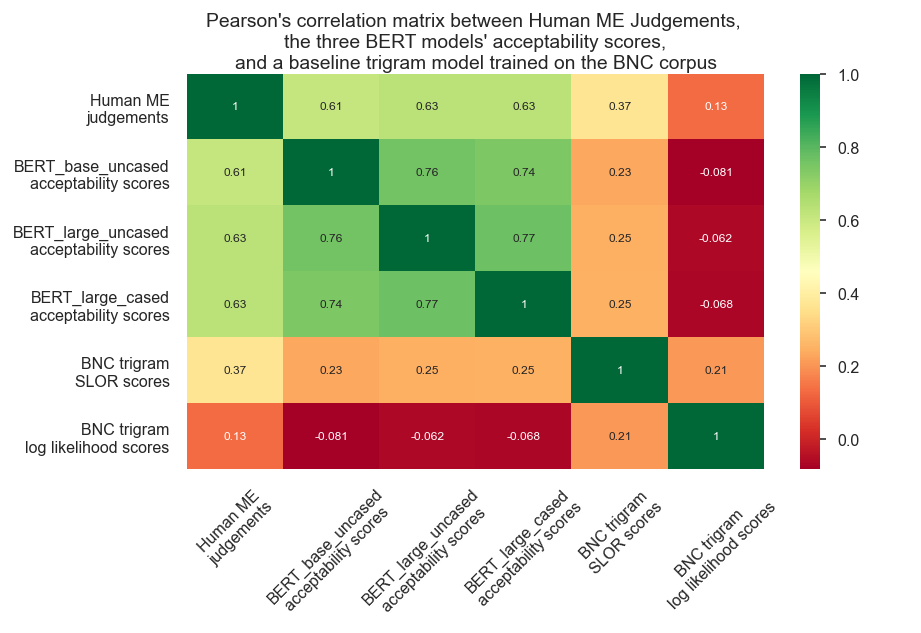
\includegraphics[scale=0.5]{templates/figures/bert_acc_correlation_matrix.png}
    }
    \caption[PCC matrix between human judgements, BERT$_\mathrm{CoLA}$, \newline and a trigram model]{PCC matrix between human judgements and all three BERT$_\mathrm{CoLA}$ models.  In addition we add the SLOR and log likelihood scores of a trigram model trained on the British National Corpus by Sprouse et al. 2018 for additional reference.  All correlations shown have a $p$ < 0.0001.}
    \label{fig:bert_acc_correlation_matrix}
\end{figure}

At first glance, the three BERT$_\mathrm{CoLA}$ models have a moderate positive correlation of slightly above 0.6 with the human judgements on the LI-Adger dataset.  However, upon closer inspection, it quickly becomes apparent that this summary statistic can be deceptive.  We show in Figure \ref{fig:bert_acc_correlation_plot} a scatterplot of the BERT$_\mathrm{CoLA}$ models' predictions as the \textit{x} coordinate and the human judgements as the \textit{y} coordinate. 

\begin{figure}[h]
    %\centering
    \makebox[\textwidth][c]{
        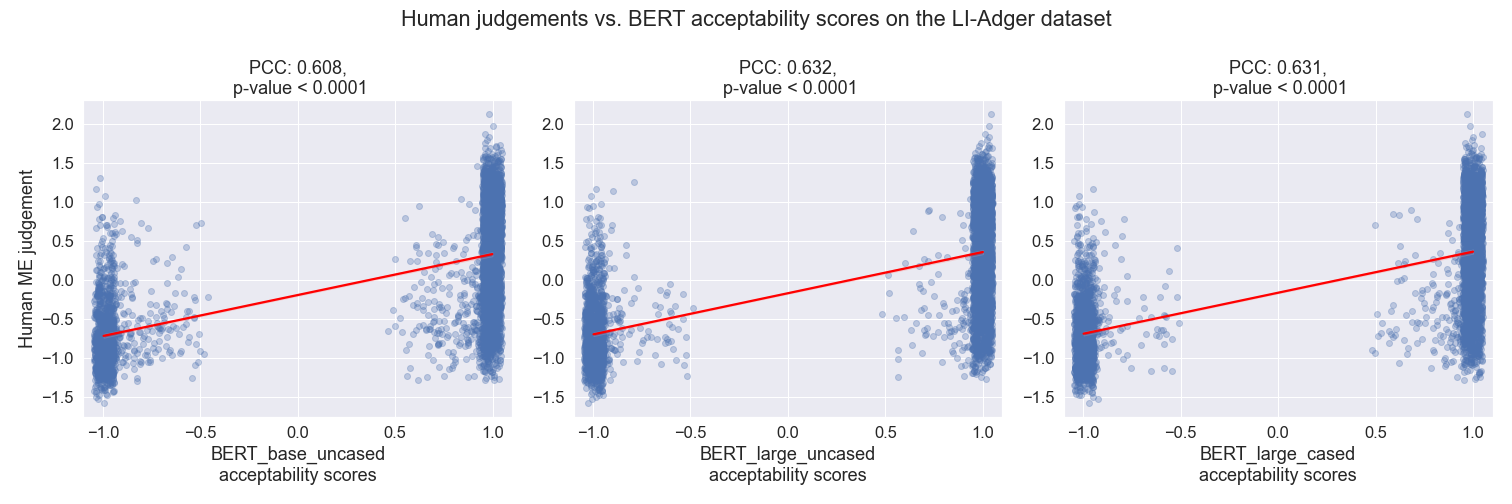
\includegraphics[scale=0.3]{templates/figures/bert_acc_correlation_plot.png}
    }
    \caption[Human judgements vs. BERT$_\mathrm{CoLA}$ acceptability scores \newline on LI-Adger dataset]{Scatterplot of human judgements (\textit{y}-axis) vs. BERT$_\mathrm{CoLA}$ acceptability score output for each sentence in the LI-Adger dataset with best-fit line in red.  We add a jitter of 0.05 along the \textit{x}-axis and lower the alpha to 0.3 to highlight the density of the points.}
    \label{fig:bert_acc_correlation_plot}
\end{figure}

Figure \ref{fig:bert_acc_correlation_plot} shows how, despite a PCC of $>0.6$ across all three BERT$_\mathrm{CoLA}$ models, they all fail to capture the full range of possible acceptability scores.  In fact, it seems that the three BERT$_\mathrm{CoLA}$ models, contrary to our expectations, mostly only output acceptability scores either greater than $0.9$ or less than $-0.9$.  We believe there are at least two (but likely more) possible sources of this behavior.  This may be a symptom of the underspecification observed in \ref{section:bert_instability}, where the free parameters have led BERT$_\mathrm{CoLA}$ to effectively \textit{memorize} the categorical labels instead of generalizing to gradient acceptability values.  The other possible explanation could be that the softmax output from Equation \ref{eqn:bert_softmax} is consistently overestimating the label probabilities, either because the output layer was not calibrated as per \citet{guo2017calibration}, or the learned weight embedding matrix $W$ is unable to map the encoded output of BERT$_\mathrm{CoLA}$'s final hidden layer to the acceptability gradient.  We do not take a stance as to what the cause of the behavior may be, and merely use it to have an idea of what to expect from the three BERT$_\mathrm{CoLA}$ models when we apply the Acceptability Delta Criterion.

\section{BERT takes on the ADC (ADC round 1)}

In light of how the three BERT$_\mathrm{CoLA}$ models fail to account for the full range of acceptability values in the LI-Adger dataset, the three models now become a good case study of how well the Acceptability Delta Criterion (ADC) may be able to discern this.  As a brief reminder, the ADC requires that the model outputs be Z-score transformed such that they are expressed in terms of standard deviation units.  Afterward, the LI-Adger sentences are assembled into minimal pairs, with each minimal pair ($m_i$) being associated to an Acceptability Delta from the human judgements ($\Delta h_i$) and from the models' Z-score transformed outputs ($\Delta lm_i$).  Then, if the distance between $\Delta h_i$ and $\Delta lm_i$ is greater than $\delta$ (Equation \ref{eqn:acceptability_delta_criterion_b}) or if $\Delta h_i$ and $\Delta lm_i$ differ in sign (Equation \ref{eqn:acceptability_delta_criterion_b}), the ADC for $m_i$ is not met.  For further details on the principles underlying the ADC, we refer the reader to \ref{section:acceptability_delta_criterion}.

For the remainder of this section, we will apply the ADC on the three BERT$_\mathrm{CoLA}$ models to output acceptability scores over whole sentences.  In addition, we include into our analysis the SLOR and log likelihood scores of a trigram model trained on the BNC by Sprouse et al. 2018 as a baseline.

\subsection{Correlations at the minimal pair level}
\label{section:2.5.1}
The first step in observing how the ADC may perform with the BERT$_\mathrm{CoLA}$ models and the trigram baseline is to update the PCCs using the acceptability deltas (i.e. $\Delta lm_i$) at the minimal pair level, instead of the raw acceptability scores at the individual sentence level.  Note that we will first Z-score transform the raw acceptability output from the BERT$_\mathrm{CoLA}$ models and the trigram model before computing the deltas.  This preliminary step does not affect the correlations because, as discussed at length in Section \ref{section:acceptability_delta_criterion}, the Z-score transformation is a linear operation that does not introduce distortion into the data (\citealp{schutze},pp 27-51).  We recreate in Figure \ref{fig:bert_acc_correlation_matrix} an updated correlation matrix using the newly computed acceptability deltas from the six metrics compared in Section \ref{section:2.4}.


\begin{figure}[h]
    %\centering
    \makebox[\textwidth][c]{
        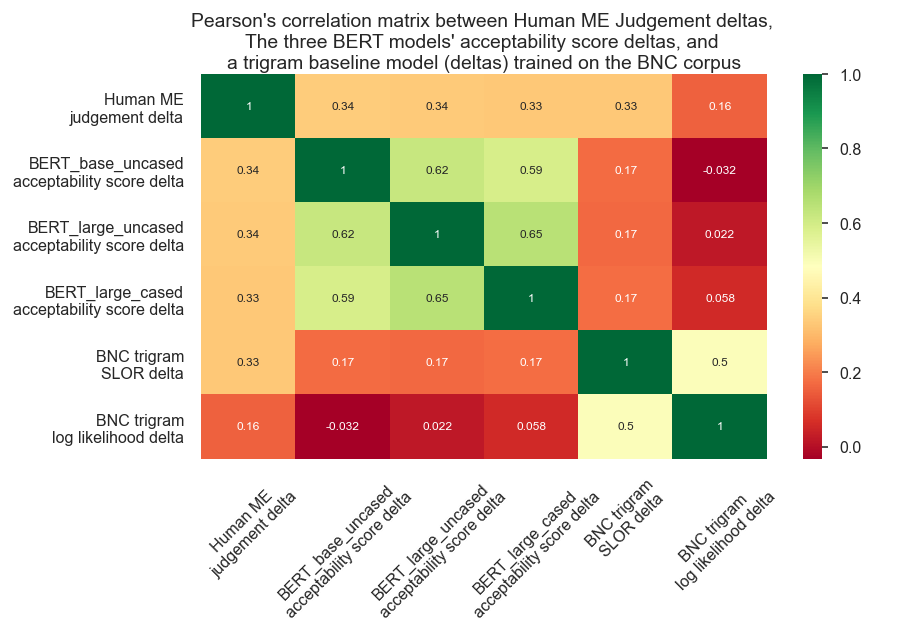
\includegraphics[scale=0.5]{templates/figures/bert_acc_delta_correlation_matrix.png}
    }
    \caption[PCC matrix between human judgements, BERT$_\mathrm{CoLA}$, \newline and a trigram model]{PCC matrix between human judgements and all three BERT$_\mathrm{CoLA}$ models.  In addition we add the SLOR and log likelihood scores of a trigram model trained on the British National Corpus by Sprouse et al. 2018 for additional reference.  All correlations shown have a $p$ < 0.0001.}
    \label{fig:bert_acc_delta_correlation_matrix}
\end{figure}

We see a precipitous drop in the PCCs between the human data and the three BERT$_\mathrm{CoLA}$ models, yet the trigram model's PCCs remain relatively constant.  This lends credence to the idea that the source of the moderate to strong positive correlation observed in Section \ref{section:2.4} was a result of the same spurious correlations causing the instability in Section \ref{section:bert_instability}.  For ease of comparison, we present in Table \ref{tab:table_8} the PCCs between the human judgement data and the 5 models currently under study at the individual sentence level and at the minimal pair (delta) level. 

\begin{table}[h]
    \centering
    \ra{1.3}
    \begin{tabular}{@{}lcc@{}}
    \toprule
    \textbf{Model} & \textbf{PCC LI-Adger sentences} & \textbf{PCC LI-Adger min pairs}  \\
    \midrule
    BERT$_\mathrm{CoLA_{base-uncased}}$ & 0.608 & 0.340 \\
    BERT$_\mathrm{CoLA_{large-uncased}}$ & 0.632 & 0.338 \\
    BERT$_\mathrm{CoLA_{large-cased}}$ & 0.631 & 0.335 \\
    \midrule
    trigram$_{SLOR}$ & 0.368 & 0.333 \\
    trigram$_{log-prob}$ & 0.131 & 0.156 \\
    \bottomrule
    \end{tabular}
    \caption[PCCs with human data on LI-Adger sentences vs. minimal pairs]{PCCs on the LI-Adger dataset on invididual sentences (middle) and across minimal pairs (right) between human acceptability judgements and 5 other models.  We include three BERT$_\mathrm{CoLA}$ models, as well as SLOR and log-likelihood scores from a trigram model trained on the British National Corpus by Sprouse et al. 2018}
    \label{tab:table_8}
\end{table}

To conclude this section, we redraw the correlation plots with best-fit lines from Section \ref{section:2.4} but now using the acceptability delta values at the minimal pair level.  Figure \ref{fig:bert_acc_delta_correlation_plot} confirms our suspicions regarding the BERT$_\mathrm{CoLA}$ models' behavior: despite our reformulation of BERT$_\mathrm{CoLA}$ models' outputs in order to make them gradient in line with human acceptability judgements, the models consistently predicted sentences to be either more than 90\% acceptable or less than 90\% unacceptable.

\begin{figure}[h]
    %\centering
    \makebox[\textwidth][c]{
        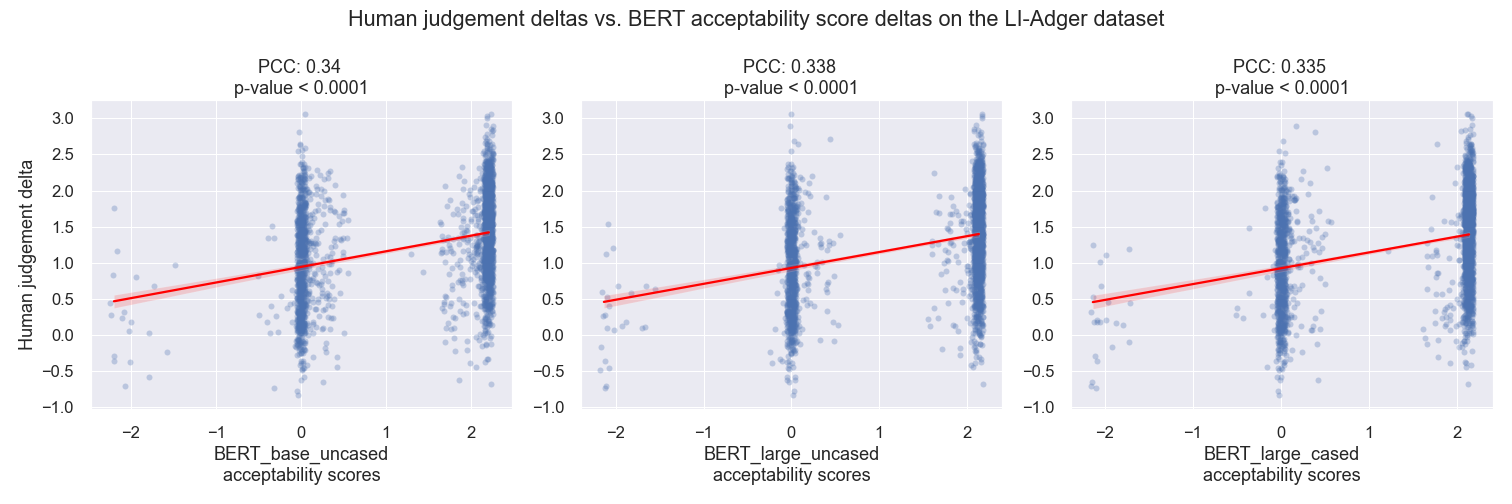
\includegraphics[scale=0.3]{templates/figures/bert_acc_delta_correlation_plot.png}
    }
    \caption[Human judgement deltas vs. BERT$_\mathrm{CoLA}$ acceptability \newline score deltas on LI-Adger minimal pairs]{Scatterplot of human judgement deltas (\textit{y}-axis) vs. BERT$_\mathrm{CoLA}$ acceptability score deltas for each minimal pair in the LI-Adger dataset with best-fit line in red.  We add a jitter of 0.05 along the \textit{x}-axis and lower the alpha to 0.3 to highlight the density of the points.}
    \label{fig:bert_acc_delta_correlation_plot}
\end{figure}

Despite our best efforts to have $BERT_{\mathrm{CoLA}}$ output gradient acceptability judgements with the formulation discussed in Equation \ref{eqn:bert_softmax}, the fine-tuning phase on categorical data only seems to cripple the models' performance, contrary to our expectations as discussed in \ref{section:2.1}.  What we find most surprising is not the precipitous drop in PCC when considering a simple delta across a minimal pair, but that the PCC was at the level of that of a trigram model.  We investigate this further by studying the three BERT$_\mathrm{CoLA}$ models' performance under the ADC, comparing them against the trigram baseline.

\subsection{Applying the Acceptability Delta Criterion}
\label{section:2.5.2}
Here we conduct one final analysis of the BERT$_\mathrm{CoLA}$ models.  We benchmark the three models as well as the two trigram metrics using the BLiMP Criterion and the ADC using three different values of $\delta$.  We use $\delta=0.5$ as the strictest test, requiring that the LM acceptability delta ($\Delta lm_i$) and the human judgement delta ($\Delta h_i$) be within 0.5 standard deviation units of each other.  Increasing $\delta$ makes the test progressively easier, until it functionally becomes very similar to the BLiMP criterion, with the crucial difference being that the BLiMP Criterion maintains the expert labels as the ground truth, whereas the ADC will use the sign of the human judgements as the true label of each sentence.

In order to test how the ADC generalizes to a form similar to the BLiMP criterion, we add two additional ADC tests: one with $\delta=1$ and one with $\delta=5$.  We report the results of our 4 tests in Table \ref{tab:table_9}.



\begin{table}[h]
    \centering
    \ra{1.3}
    \begin{tabular}{@{}lcccc@{}}
    \toprule
    \textbf{Model} & \textbf{BLiMP} & \textbf{ADC, $\delta=0.5$} & \textbf{ADC, $\delta=1.0$} & \textbf{ADC, $\delta=5.0$}  \\
    \midrule
    BERT$_\mathrm{CoLA_{base-uncased}}$ & 0.915 & 0.286 & 0.538 & 0.902\\
    BERT$_\mathrm{CoLA_{large-uncased}}$ & 0.917 & 0.311 & 0.564 & 0.907 \\
    BERT$_\mathrm{CoLA_{large-cased}}$ & 0.936 & 0.307 & 0.561 & 0.925\\
    \midrule
    trigram$_{SLOR}$ & 0.753 & 0.301 & 0.520 & 0.744\\
    trigram$_{log-prob}$ & 0.671 & 0.165 & 0.329 & 0.668 \\
    \bottomrule
    \end{tabular}
    \caption[BERT$_\mathrm{CoLA}$ and trigram model scores under BLiMP \& ADC]{Comparison between the models' BLiMP and ADC scores, using $\delta$=\{0.5, 1.0, 5.0\}. We include three BERT$_\mathrm{CoLA}$ models, as well as SLOR and log-likelihood scores from a trigram model trained on the British National Corpus by Sprouse et al. 2018}
    \label{tab:table_9}
\end{table}

The initial results of the ADC are very promising.  For one, the BERT$_\mathrm{CoLA}$ model scores under $\delta=0.5$ are in line with our expectations from the PCCs observed in Section \ref{section:2.5.1}.  This is supported by the trigram's SLOR performance also under the ADC with $\delta=0.5$, which is also extremely close to the BERT$_\mathrm{CoLA}$ models' PCCs at the minimal pair level.  It is also a promising sign to see that the BERT$_\mathrm{CoLA}$ model scores and the trigram SLOR scores scale together at $\delta = 1.0$.  Lastly, setting $\delta=5.0$ as a large number yielded scores for all 5 models very close to their performance under the BLiMP Criterion, strongly suggesting that the ADC is in fact a generalization of the BLiMP criterion when the stricter $\delta$ measure is relaxed.  Testing this further, we present 4 example minimal pairs that BERT$_\mathrm{CoLA_{large-cased}}$ scored correctly under the BLiMP Criterion, but not under the ADC with $\delta=5.0$ in Table \ref{tab:table_10}.

\begin{table}[h]
    \centering
    \ra{1.3}
    \begin{tabular}{@{}lcc@{}}
    \toprule
    \textbf{Minimal Pair} & Human & BERT\\
    \textbf{Top}: Acceptable | \textbf{Bottom}: Unacceptable & judgement & acceptability\\
    \toprule
    We proved Amelia to the manager to be responsible.  & -0.56008 & 0.732817911 \\
    *We proved to the manager Amelia to be responsible. & -0.13864 & -1.39757562 \\
    \midrule
    There is likely to live a snake in the garden. & -0.6451 & -1.02182 \\
    *There is likely a snake to live in the garden.   &  -0.51201 & -1.39602 \\
    \midrule
    Jenny would accurately have calculated the results. & 0.345683 & -1.340338319 \\
    *Jenny accurately will calculate the results.  & 0.501494 & -1.40060934 \\
    \midrule
    The announcer's introduction of Ted was humorous.  & 0.659471 & 0.73306608 \\
    The announcer's introduction of Ted's was humorous. & 0.748718 & -1.335794047 \\
    \bottomrule
    \end{tabular}
    \caption[Four minimal pairs where the BLiMP Criterion and \newline ADC with $\delta=5.0$ differ]{Four minimal pairs where the BERT$_\mathrm{CoLA}$ models meet the BLiMP Criterion but not the generalized ADC with $\delta=5.0$. We report the BERT acceptability score from BERT$_\mathrm{CoLA_{large-cased}}$ The human judgement and BERT acceptability scores are already z-score transformed.  The common factor is that the human judgements disagree with the BLiMP Criterion.}
    \label{tab:table_10}
\end{table}

The common factor among the four minimal pairs presented in Table \ref{tab:table_10}, and the other 54 minimal pairs where BERT$_\mathrm{CoLA_{large-cased}}$ fulfilled the BLiMP criterion but not the ADC with $\delta=5$, is that the human judgements disagree with the expert categorization.  This is, by design, one of the crucial properties of the ADC, because ultimately linguistic theory is developed by probing either language use or language acquisition.  

%Table \ref{tab:table_10} four different minimal pairs that highlight where the BLiMP Criterion and the generalized ADC overlap and where they differ.
%\begin{table}[h]
%    \centering
%    \ra{1.3}
%    \begin{tabular}{@{}cll@{}}
%    \toprule
%    \textbf{Criteria Met} & \textbf{Minimal Pair IDs} & \textbf{Minimal Pair} \\
%    \midrule
%    Both BLiMP  & 32.1.martin.66a.g.03 & It is important for one to sleep regularly.\\
%    and ADC & 32.1.martin.66b.*.03 & It is important one to sleep regularly. \\
%    \midrule
%    Only BLiMP & 35.3.hazout.67a.g.06 & There is likely to live a snake in the garden. \\
%    & 35.3.hazout.67c.*.06 & There is likely a snake to live in the garden. \\
%    \midrule
%    Only ADC & 35.3.richards.17a.g.03 & What did you send to whom? \\
%    & 35.3.richards.17b.*.03 & To whom did you send what? \\
%    \midrule
%    Neither BLiMP  & ch10.84-86.g.03 & What did Kelly watch a TV show about? \\
%    nor ADC & ch10.83.*.03 & What did Kelly watch those TV shows about? \\
%    \bottomrule
%    \end{tabular}
%    \caption[Example minimal pairs highlighting where the BLiMP and ADC with $\delta=5.0$ criteria overlap and differ]{Example minimal pairs that meet both, either the BLiMP Criterion or the generalized ADC with $\delta=5.0$, or neither criteria.}
%    \label{tab:table_10}
%\end{table}

%\todo[inline]{Some observation about the above table.}

With a clearer idea of the difference between the BLiMP Criterion and the generalized ADC, one big question remains: how much overlap is there between the performance of the trigram model and the BERT$_\mathrm{CoLA}$ models?  In other words, is it purely coincidental that all three BERT$_\mathrm{CoLA}$ models and the trigram SLOR scores had extremely close PCCs on the acceptability deltas \textbf{and} extremely close scores on the ADC for both $\delta=0.5$ and $\delta=1.0$?  If we consider that $N$-gram class models have little to no KoL other than word cooccurrence, and that the BERT$_\mathrm{CoLA}$ models did not seem to track sentences across the acceptability spectrum, this is a question that demands at least some cursory sanity checks.  Accordingly, we perform two more evaluations of the ADC but with different datasets.  For the first, we use the results for the ADC with $\delta=0.5$ from Table \ref{tab:table_9} to subtract from the LI-Adger dataset all the minimal pairs where the trigram SLOR deltas met the ADC.  We hope that by doing so, we will have factored out from the dataset all the minimal pairs that can be correctly tracked using purely word cooccurrence statistics, thereby leaving behind only minimal pairs whose acceptability delta requires the BERT$_\mathrm{CoLA}$ models' extra machinery (parameters) to correctly track.  Table \ref{tab:table_11} presents the BERT$_\mathrm{CoLA}$ models' scores under the ADC with $\delta$=\{0.5,1.0\} before and after removing the minimal pairs where the trigram SLOR model met the ADC. 

%\begin{table}[h]
    %\centering
    %\ra{1.3}
    %\begin{tabular}{@{}cccc@{}}
    %\toprule
    %\textbf{Model} & \textbf{ADC, $\delta=0.5$} & \textbf{ADC, %$\delta=0.5$} & \textbf{Total} \\
                   %& \textbf{original}          & \textbf{sans trigram}      & \textbf{overlap}\\
    %\midrule
    %BERT$_{base-uncased}$ & 0.286 & 0.294 & 8.08\% \\
    %BERT$_{large-uncased}$ & 0.311 & 0.309 & 9.51\% \\
    %BERT$_{large-cased}$ & 0.307 & 0.313 & 8.84\% \\
    %\bottomrule
    %\end{tabular}
    %\caption[BERT models' ADC with $\delta=0.5$ scores sans easy min pairs]{BERT models' performance on the ADC with $\delta=0.5$ before and after removing all minimal pairs for which the ADC Criterion was met by the trigram baseline model trained on the BNC corpus. The third column is the percentage of BERT's passing minimal pairs that the trigram baseline also passed.}
    %\label{tab:table_11}
%\end{table}


%\begin{table}[h]
    %\centering
    %\ra{1.3}
    %\begin{tabular}{@{}cccc@{}}
    %\toprule
    %\textbf{Model} & \textbf{ADC, $\delta=1.0$} & \textbf{ADC, %$\delta=1.0$} & \textbf{Total}\\
                   %& \textbf{original}          & \textbf{sans trigram}      & \textbf{overlap}\\
    %\midrule
    %BERT$_{base-uncased}$ & 0.538 & 0.546 & 27.6\% \\
    %BERT$_{large-uncased}$ & 0.564 & 0.557 & 29.6\% \\
    %BERT$_{large-cased}$ & 0.561 & 0.560 & 29.2\% \\
    %\bottomrule
    %\end{tabular}
    %\caption[BERT models' ADC with $\delta=1.0$ scores sans easy min pair]{BERT models' performance on the ADC with $\delta=1.0$ before and after removing all minimal pairs for which the ADC Criterion was met by the trigram baseline model trained on the BNC corpus. The third column is the percentage of BERT's passing minimal pairs that the trigram baseline also passed.}
    %\label{tab:table_12}
%\end{table}

\begin{table}[h]
    \centering
    \ra{1.3}
    \begin{tabular}{@{}lcccccc@{}}
    \toprule
    \textbf{Model} & \multicolumn{3}{c}{\textbf{ADC, $\delta=0.5$}} &  \multicolumn{3}{c}{\textbf{ADC, $\delta=1.0$}} \\
    \cmidrule{2-3} \cmidrule{4-7}
    \textbf{BERT$_\mathrm{CoLA}$} & \textbf{Original} & \textbf{Reduced} & \textbf{Overlap} & \textbf{Original} & \textbf{Reduced} & \textbf{Overlap} \\
    \midrule
    base-uncased & 0.286 & 0.294 & 8.08\% & 0.538 & 0.546 & 27.6\%\\
    large-uncased & 0.311 & 0.309 & 9.51\% & 0.564 & 0.557 & 29.6\%\\
    large-cased & 0.307 & 0.313 & 8.84\% &  0.561 & 0.560 & 29.2\% \\
    \bottomrule
    \end{tabular}
    \caption[BERT$_\mathrm{CoLA}$ ADC with $\delta=$\{0.5,1.0\} scores \newline sans easy min pairs]{BERT$_\mathrm{CoLA}$ models' performance on the ADC with $\delta$={0,5,1.0} before (Original) and after (Reduced) removing all minimal pairs for which the ADC Criterion was met by the trigram baseline model trained on the BNC corpus. The Overlap columns display the percentage of minimal pairs that both the BERT$_\mathrm{CoLA}$ model and the trigram baseline pass.}
    \label{tab:table_11}
\end{table}

Poor performance aside, Table \ref{tab:table_11} reveals a small change in overall performance and a low percentage of minimal pairs correctly scored by both the BERT$_\mathrm{CoLA}$ models and the trigram model using SLOR.  This allays concerns that the BERT$_\mathrm{CoLA}$ models might only be doing well on minimal pairs that the trigram model also predicts correctly.  To conclude, we inspect a few example minimal pairs that all three BERT$_\mathrm{CoLA}$ models scored correctly but the trigram did not (Table \ref{tab:table_13}), and vice versa: a few example minimal pairs the trigram model scored correctly using SLOR but none of the three BERT$_\mathrm{CoLA}$ models did (Table \ref{tab:table_14}).

\begin{table}[h]
    \centering
    \ra{1.3}
    \begin{tabular}{@{}lcc@{}}
    \toprule
    \textbf{Minimal Pair}                                    & trigram   & BERT$_\mathrm{CoLA}$\\
    \textbf{Top}: Acceptable | \textbf{Bottom}: Unacceptable & SLOR      & acceptability\\
    \toprule
    She taught the students math.  & -0.685949 & 0.73276 \\
    *She taught math the students. & -0.562807 & -1.40171 \\
    \midrule
    There are linguists available. & -0.337031 & 0.732224 \\
    *There are linguists tall.     &  -0.512287 & -1.41472 \\
    \midrule
    Our professor gave no extensions to any students. & -0.728557 & 0.721394 \\
    *Our professor gave any extensions to no students.  & -1.33971 & -1.3493 \\
    \midrule
    What did you address to whom?  & 0.478869 & 0.73067 \\
    *To whom did you address what? & -0.890322 & 0.681159 \\
    \bottomrule
    \end{tabular}
    \caption[Four minimal pairs where BERT$_\mathrm{CoLA}$ meets ADC\newline with $\delta=0.5$ but not the trigram model]{Four minimal pairs where all BERT$_\mathrm{CoLA}$ models meet the ADC with $\delta=0.5$ but the trigram baseline does not. We report the acceptability score from BERT$_\mathrm{CoLA_{large-cased}}$. The trigam SLOR and BERT$_\mathrm{CoLA_{large-cased}}$ acceptability scores are already z-score transformed. }
    \label{tab:table_13}
\end{table}

\begin{table}[h]
    \centering
    \ra{1.3}
    \begin{tabular}{@{}lcc@{}}
    \toprule
    \textbf{Minimal Pair}                                    & trigram   & BERT$_\mathrm{CoLA}$\\
    \textbf{Top}: Acceptable | \textbf{Bottom}: Unacceptable & SLOR      & acceptability\\
    \toprule
    Michael managed to drive his car.  & 0.950214 & 0.733175 \\
    *Michael managed to have driven his car. & 0.26957 & -1.37701 \\
    \midrule
    Paul flew to Ireland and Laura sailed to Greece. & 0.253906 & 0.733086 \\
    *Paul flew Ireland and Laura sailed to Greece. &  -0.779695 & 0.731989 \\
    \midrule
     She ran into Spencer and asked him out. &  0.821345 & 0.73299 \\
    *She ran into Spencer and asked out.  & -0.194269 & -1.38959 \\
    \midrule
    The children are almost all sleeping.  & 0.30149 & 0.733162 \\
    The children almost all are sleeping. & -0.680258 & 0.729437 \\
    \bottomrule
    \end{tabular}
    \caption[Four minimal pairs where the trigram model meets ADC \newline with $\delta=0.5$ but not BERT$_\mathrm{CoLA}$]{Four minimal pairs where the trigram baseline meets the ADC with $\delta=0.5$ but none of the BERT models do. We report the BERT acceptability score from BERT$_\mathrm{CoLA_{large-cased}}$. The trigam SLOR and BERT$_\mathrm{CoLA_{large-cased}}$ acceptability scores are already z-score transformed. }
    \label{tab:table_14}
\end{table}

Taking Table \ref{tab:table_13} as the only source of evidence, it seems the trigram model is failing to meet the ADC when the words in the unacceptable sentence of the minimal pair are okay locally, but result in a very overtly bad sentence.  The main exception would perhaps be the last example in \ref{tab:table_13}, in which the BERT$_\mathrm{CoLA}$ models correctly agreed with the human judgements that both sentences of the pair are okay.  The trigram model likely struggled with the frequency imbalance between \textit{What} and \textit{To whom} at the start and end of both sentences.

However, the BERT$_\mathrm{CoLA}$ models' lack of gradience is revealed when considering Table \ref{tab:table_14}.  Most of the BERT$_\mathrm{CoLA_{large-cased}}$'s predictions shown in Tables \ref{tab:table_10}, \ref{tab:table_13} and \ref{tab:table_14} are either very unacceptable ($\sim$-1.3) or very acceptable ($\sim 0.7$).  Precisely this behavior is what causes the BERT$_\mathrm{CoLA}$ models to have such a low performance under the ADC, and such low PCCs in Section \ref{section:2.5.1}.  This is made even clearer when considering the third minimal pair in Table \ref{tab:table_14}: both the trigram and BERT$_\mathrm{CoLA}$ agree in the sign of their predictions, but BERT$_\mathrm{CoLA}$ predicts a shift from completely unacceptable to completely acceptable, unlike the trigram whose acceptability delta is more moderate.  This leads the trigram to fall within the 0.5 standard deviation units required by ADC with $\delta=0.5$, whereas the three BERT$_\mathrm{CoLA}$ models do not.

